\documentclass{article}
\usepackage{ae,aecompl}
\usepackage{todonotes}
\usepackage{chngcntr}
\usepackage{tikz-cd}
\usepackage{graphicx}
\graphicspath{ {./images/}}
\usepackage[all,cmtip]{xy}
\usepackage{amsmath, amscd}
\usepackage{amsthm}
\usepackage{amssymb}
\usepackage{amsfonts}
\usepackage{bm}
\usepackage{qsymbols}
\usepackage{latexsym}
\usepackage{mathrsfs}
\usepackage{mathtools}
\usepackage{cite}
\usepackage{color}
\usepackage{url}
\usepackage{enumerate}
\usepackage{verbatim}
\usepackage[draft=false, colorlinks=true]{hyperref}
\usepackage{pdfpages}
\usepackage[margin=1.2in]{geometry}
\usepackage{IEEEtrantools}

\usepackage{fancyhdr}


\usepackage[nameinlink]{cleveref}


\DeclareMathOperator*{\ac}{accept}
\DeclareMathOperator*{\amax}{argmax}
\DeclareMathOperator*{\amin}{argmin}
\DeclareMathOperator*{\Aut}{Aut}
\newcommand {\al}{{\alpha}}
\newcommand {\abs}[1]{{\left\lvert#1\right\rvert}}
\newcommand {\A}{{\mathcal{A}}}
\newcommand {\AM}{{\mathrm{AM}}}
\newcommand {\AMp}{{\AM_{p}^{X}\!(\Ri_\w)}}
\newcommand {\B}{{\mathcal{B}}}
\DeclareMathOperator*{\Be}{Bern}
\newcommand {\Br}{{\dot{B}}}
\newcommand {\Ba}{{\mathfrak{B}}}
\newcommand {\C}{{\mathbb C}}
\newcommand {\ce}{\mathrm{c}}
\newcommand {\Ce}{\mathrm{C}}
\newcommand {\Cc}{\mathrm{C_{c}}}
\newcommand {\Ccinf}{\mathrm{C_{c}^{\infty}}}
\DeclareMathOperator{\cov}{Cov}
\DeclareMathOperator{\DEV}{DEV}
\newcommand {\Di}{{\mathbb D}}
\newcommand {\dom}{\mathrm{dom}}
\newcommand{\dist}{\stackrel{\mathrm{dist}}{=}}
\newcommand {\ud}{\mathrm{d}}
\newcommand {\ue}{\mathrm{e}}
\newcommand {\eps}{\varepsilon}
\newcommand {\veps}{\varepsilon}
\newcommand {\vrho}{{\varrho}}
\newcommand {\E}{{\mathbb{E}}}
\newcommand {\Ec}{{\mathcal{E}}}
\newcommand {\Ell}{L}
\newcommand {\Ellp}{{L_{p}[0,1]}}
\newcommand {\Ellpprime}{{L_{p'}([0,1])}}
\newcommand {\Ellq}{{L_{q}([0,1])}}
\newcommand {\Ellqprime}{{L_{q'}([0,1])}}
\newcommand {\Ellr}{L^{r}}
\newcommand {\Ellone}{{L_{1}([0,1])}}
\newcommand{\Elltwo}{{L_{2}([0,1])}}
\newcommand{\Ellinfty}{L^{\infty}}
\newcommand{\Ellinftyc}{L_{\mathrm{c}}^{\infty}}
\newcommand{\exb}[1]{\exp\left\{#1\right\}}
\DeclareMathOperator*{\Ext}{Ext}
\newcommand{\F}{{\mathcal{F}}}
\newcommand{\Fe}{{\mathbb{F}}}
\newcommand{\G}{{\mathcal{G}}}
\newcommand{\HF}{\mathcal{H}_{\text{FIO}}^{1}(\Rd)}
\newcommand{\Hr}{H}
\newcommand{\HT}{\mathcal{H}}
\newcommand{\ui}{\mathrm{i}}
\newcommand{\I}{{I}}
\newcommand{\J}{{\mathcal{J}}}
\newcommand{\id}{{\mathrm{id}}}
\newcommand{\iid}{\stackrel{\mathclap{\normalfont\mbox{iid}}}{\sim}}
\newcommand{\im}{{\text{im }}}
\newcommand{\ind}{{\perp\!\!\!\perp}}
\DeclareMathOperator*{\Int}{int}
\newcommand{\intx}{{\overline{\int_{X}}}}
\newcommand{\inte}{{\overline{\int_{\E}}}}
\newcommand{\la}{\lambda}
\newcommand{\rb}{\rangle}
\newcommand{\lb}{{\langle}}
\newcommand{\La}{\Lambda}
\newcommand{\calL}{{\mathcal{L}}}
\newcommand{\lp}{{\mathcal{L}}^{p}}
\newcommand{\lpo}{{\overline{\mathcal{L}}^{p}\!}}
\newcommand{\Lpo}{{\overline{\Ell}^{p}\!}}
\newcommand{\M}{{\mathbf{M}}}
\newcommand{\Ma}{{\mathcal{M}}}
\newcommand{\N}{{{\mathbb N}}}
\newcommand{\Na}{{{\mathcal{N}}}}
\newcommand{\norm}[1]{\left\|#1\right\|}
\newcommand{\normm}[1]{{\left\vert\kern-0.25ex\left\vert\kern-0.25ex\left\vert #1 
    \right\vert\kern-0.25ex\right\vert\kern-0.25ex\right\vert}}
\newcommand{\Om}{{{\Omega}}}
\newcommand{\one}{{{\bf 1}}}
\newcommand{\pic}{\text{Pic }}
\newcommand{\ph}{{\varphi}}
\newcommand{\Pa}{{\mathbb{P}}}
\newcommand{\Po}{{\mathcal{P}}}
\newcommand{\Q}{{\mathbb{Q}}}
\newcommand{\R}{{\mathbb R}}
\newcommand{\Rd}{{\mathbb{R}^{d}}}
\DeclareMathOperator{\rej}{reject }
\newcommand{\Rn}{{\mathbb{R}^{n}}}
\newcommand{\cR}{{\mathcal{R}}}
\newcommand{\Rad}{{\mathrm{Rad}}}
\newcommand{\ran}{{\mathrm{ran}}}
\newcommand{\Ri}{{\mathrm{R}}}
\newcommand{\supp}{{\mathrm{supp}}}
\newcommand{\Se}{\mathrm{S}}
\newcommand{\Sp}{S^{*}(\Rn)}
\newcommand{\St}{{\mathrm{St}}}
\newcommand{\Sw}{\mathcal{S}}
\newcommand{\T}{{\mathcal{T}}}
\newcommand{\ta}{{\theta}}
\newcommand{\Ta}{{\Theta}}
\newcommand{\topp}{\stackrel{p}{\to}}
\newcommand{\todd}{\stackrel{d}{\to}}
\newcommand{\toL}[1]{\stackrel{L^{#1}}{\to}} 
\newcommand{\toas}{\stackrel{a.s.}{\to}}
\DeclareMathOperator{\V}{Var}
\newcommand {\w}{{\omega}}
\newcommand {\W}{{\mathrm{W}}}
\newcommand {\Wnp}{\text{$\mathrm{W}$\textsuperscript{$n,\!p$}}}
\newcommand {\Wnpeq}{\text{$\mathrm{W}$\textsuperscript{$n\!,\!p$}}}
\newcommand {\Wonep}{\text{$\mathrm{W}$\textsuperscript{$1,\!p$}}}
\newcommand {\Wonepeq}{\text{$\mathrm{W}$\textsuperscript{$1\!,\!p$}}}
\newcommand {\X}{{\mathcal{X}}}
\newcommand {\Z}{{{\mathbb Z}}}
\newcommand {\Za}{{\mathcal{Z}}}
\newcommand {\Zd}{{\Z[\sqrt{d}]}}
\newcommand {\vanish}[1]{\relax}

\newcommand {\wh}{\widehat}
\newcommand {\wt}{\widetilde}
\newcommand {\red}{\color{red}}

% Distributions
\newcommand{\normal}{\mathsf{N}}
\newcommand{\poi}{\mathsf{Poisson}}
\newcommand{\bern}{\mathsf{Bernoulli}}
\newcommand{\bin}{\mathsf{Binomal}}
\newcommand{\multi}{\mathsf{Multinomial}}
\newcommand{\Exp}{\mathsf{Exp}}



% put your command and environment definitions here




% some theorem environments
% remove "[theorem]" if you do not want them to use the same number sequence


  \newtheorem{thrm}{Theorem}
  \newtheorem{lemma}{Lemma}
  \newtheorem{prop}{Proposition}
  \newtheorem{cor}{Corollary}

  \newtheorem{conj}{Conjecture}
  \renewcommand{\theconj}{\Alph{conj}}  % numbered A, B, C etc

  \theoremstyle{definition}
  \newtheorem{defn}{Definition}
  \newtheorem{ex}{Example}
  \newtheorem{exs}{Examples}
  \newtheorem{question}{Question}
  \newtheorem{remark}{Remark}
  \newtheorem{notn}{Notation}
  \newtheorem{exer}{Exercise}


\newcommand{\Ss}{\mathcal{S}}

\title{STATS305A - Lecture 13}
\author{John Duchi\\ Scribed by Michael Howes}
\date{11/04/21}

\pagestyle{fancy}
\fancyhf{}
\rhead{STATS305A - Lecture 13}
\lhead{11/04/21}
\rfoot{Page \thepage}

\begin{document}
\maketitle
\tableofcontents

\section{Announcements}
\begin{itemize}
    \item Exercise 3 to be released today. 
    \item An email announcement will be sent when exercise 3 is available.
\end{itemize}
\section{Risk and model selection}
Recall that we are now looking at model selection and prediction. We are starting with the more general model $y = f(x)+\eps$ where $f(x) = \E[y|x]$ and we want to fit a predictor $h:\X \to \R$. 

We can think of having a sequence of model spaces $\HT_1 \subset \HT_2 \subset \ldots \subset \HT_k \subset \ldots$. We want to find $h$ such that the quantity 
\[\frac{1}{n}\sum_{i=1}^n(y_i-h(x_i))^2,\]
is small but $h$ is not too ``complex''. Typically we think of $\HT_k$ as growing in complexity as $k$ increases. Thus we wish to choose $h \in \HT_k$ minimizing
\[\sum_{i=1}^n(y_i-h(x_i))^2+\text{penalty}(h), \]
or 
\[\sum_{i=1}^n(y_i-h(x_i))^2+\text{penalty}(\HT_k). \]
Talking about this last time led to Mallows's $C_p$ statistic which was
\[C_p = \norm{y-X\beta}_2^2 + 2\sigma^2p, \]
where $\beta \in \R^p$ and $2\sigma^2p$ is a complexity penalty. Mallows's method is to choose the model that minimizes $C_p$.
\subsection{Bias variance tradeoff}
For any $x \in \X$ and any model procedure $\wh{h}$ we ahve 
\begin{align*}
    \E[(\wh{h}(x)-f(x))^2]&=\E\left[(\wh{h}(x)-\E[\wh{h}(x)]+\E[\wh{h}(x)]-f(x))^2\right]\\
    &=\left(\E[\wh{h}(x)]-f(x)\right)^2+\E[\left(\wh{h}(x)-\E[\wh{h}(x)]\right)^2]\\
    &=\bias(\wh{h}(x))^2+\V(\wh{h}(x)).
\end{align*}
Recall that we defined the in-sample risk to be
\[R_{in}(\wh{h}) = \frac{1}{n}\sum_{i=1}^n\E[\left(\wh{h}(x_i)-f(x_i)\right)^2], \]
where the expectation is over $Y_i = f(x_i)+\eps_i$. 
\begin{ex}
    (actually everything we will look at) Let $\mu = [f(x_i)]_{i=1}^n =\E[Y]$. Suppose 
    \[\wh{y} =Hy = [\wh{h}(x_i)]_{i=1}^n,\] 
    for some matrix $H$ that is not necessarily a projection matrix or symmetric. If $\eps \sim (0,\sigma^2I_n)$, then
    \begin{align*}
        nR_{in}(\wh{h}) &= \E\left[\norm{\wh{y}-\mu}_2^2\right]\\
        &=\E\left[\norm{Hy-\mu}_2^2\right]\\
        &=\E\left[\norm{H\mu-H\eps-\mu}_2^2\right]\\
        &=\E\left[\norm{H\eps-(I-H)\mu}_2^2\right]\\
        &=\norm{(I-H)\mu}_2^2 + \E[\norm{H\eps}_2^2]\\
        &=\bias(H)^2 + \sigma^2\tr(H^TH).
    \end{align*} 
    Likewise for the residual sum of squares (RSS) we have
    \begin{align*}
        \E[RSS] &= \E[\norm{\wh{y}-y}_2^2]\\
        &= \E[\norm{y-Hy}_2^2]\\
        &=\E[\norm{(I-H)\mu+(I-H)\eps}_2^2]\\
        &=\norm{(I-H)\mu}_2^2 + n\sigma^2-2\sigma^2 \tr(H)+\sigma^2\tr(H^TH)\\
        &=nR_{in}(\wh{h})+n\sigma^2-2\sigma^2\tr(H).
    \end{align*}
\end{ex}
\section{Ridge regression}
\subsection{Idea}
If $X$ is ``ill-conditioned'', then some errors in $y$ can induce changes in $\wh{\beta}$ that are too large if we are using OLS. 

We can formalize this with the SVD of $X$. Suppose $X = U \Gamma V^T$ is the SVD of $X$ and $\Gamma = \diag(\gamma_1,\ldots, \gamma_d)$. Then
\begin{align*}
    \wh{\beta} &= (X^TX)^{-1}X^Ty \\
    &= V\Gamma^{-1}U^Ty.
\end{align*}
Suppose $U=[u_1,\ldots, u_d] \in \R^{n \times d}$. Consider two alternative responses 
\begin{align*}
    y'&= y+tu_1,~~t \in \R,\\
    y''&=y+tu_d,~~t \in \R.
\end{align*}
We thus have 
\begin{align*}
    \wh{\beta}(y')&=\wh{\beta}(y)+\frac{tv_1}{\gamma_1}\\
    \wh{\beta}(y'') &= \wh{\beta}(y)+\frac{tv_d}{\gamma_d}.
\end{align*}
If $\gamma_d$ is very small (say $\gamma_d = \frac{1}{1000}$), then $\wh{\beta}(y'')$ will be very far from $\wh{\beta}(y)$ even if $t$ is small. This issue arises when $\frac{\gamma_1}{\gamma_d}$ is very large. The quantity $\text{cond}(X)=\frac{\gamma_1}{\gamma_d}$ is called the \emph{condition number} of $X$. In numerical analysis, $\text{cond}(X) \ge 10^6$ leads to problems. In statistics things are more sensitive and we run into trouble if $\text{cond}(X) \gtrsim 100$. 
\subsection{Ridge estimator}
One solution to the sensitivity of $\wh{\beta}$ is to regularize $\wh{\beta}$ by forcing $\Vert \wh{\beta}\Vert_2^2$ to be small.
\begin{defn}
    For $\la \ge 0$, define the \emph{ridge estimator} to be 
    \[\wh{\beta}_\la := \amin_b\left\{\norm{y-Xb}_2^2+\la\norm{b}_2^2\right\}. \]
    Since $\partial_b \left(\norm{y-Xb}_2^2+\la\norm{b}_2^2\right) = X^TXb - X^Ty+\la b$, we have that 
    \[ \wh{\beta}_\la = (X^TX+\la I)^{-1}X^Ty.\]
\end{defn}
This method of estimating $\beta$ is called ridge regression or Tikhonov regularization. 
\begin{fact}
    If $X=U\Gamma V^T$, then 
    \[\wh{y}_\la = X\wh{\beta}_\la = \sum_{j=1}^d \frac{\gamma_j^2}{\gamma_j^2+\la}u_ju_j^Ty = H_\la y, \]
    where 
    \[H_\la = U\diag\left(\frac{\gamma_j^2}{\gamma_j^2+\la}\right)U^T. \]
    Also 
    \[\frac{\partial}{\partial \la} R_{in}(\wh{\beta}_\la)|_{\la = 0} = -\frac{2\sigma^2\tr(\Gamma^{-2})}{n} < 0. \]
\end{fact}
Some thoughts on the above facts before we prove them. The normal OLS estimator satisfies 
\begin{align*}
    \wh{y} &=Hy\\
    &=UU^Ty\\
    &=\sum_{j=1}^d u_ju_j^Ty \\
    &=\Pi_{\range(X)} y.
\end{align*}
On the other hand $\wh{y}_\la$ is the projection of $y$ onto $\range(X) = \spn\{u_i\}$ but then shrunk by $\frac{\gamma_j^2}{\gamma_j^2+\la}$. The function $\gamma_j \mapsto \frac{\gamma_j^2}{\gamma_j^2+\la}$ looks like this ($\la = 4$ was used in this plot):
\begin{center}
    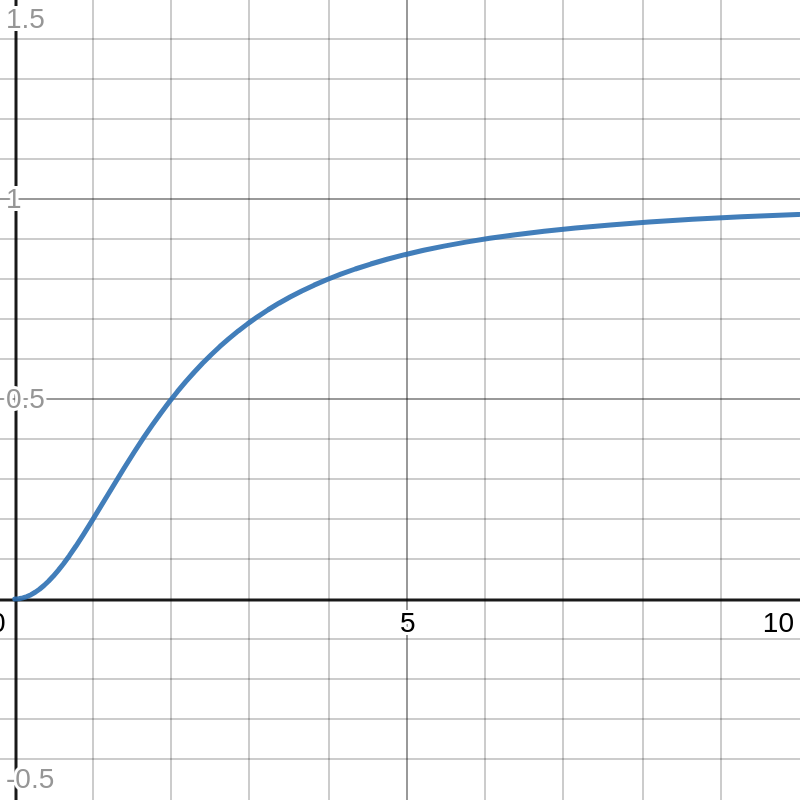
\includegraphics[width = \textwidth/2]{11_04_P01.png}
\end{center}
When $\gamma_j = 0$, $\frac{\gamma_j^2}{\gamma_j^2+\la}=0$ and as $\gamma_j \to \infty$, $\frac{\gamma_j^2}{\gamma_j^2+\la} \to 1$. When $\gamma_j = \sqrt{\la}$, $\frac{\gamma_j^2}{\gamma_j^2+\la} = \frac{1}{2}$. The idea is that for small values of $\gamma_j$, there is too much variance and we shrink away. When $\gamma_j$ is large we have lot of ``juice'' in that direction and we do not shrink much.
\begin{remark}
    In the above we are shrinking towards 0 but typically we either replace $y$ with $y-\bar{y}\one$ or use 
    \[\wh{\beta}_\la = \amin_{(b_0,b)}\left\{\norm{Xb+b_0\one - y}_2^2 + \la\norm{b}_2^2\right\}. \]
    Either of these changes mean that we shrink toward $\bar{y}$ instead of 0 and we do not regularize the intercept term. Note that if we replace $y$ with $y-\bar{y}\one$, our estimator becomes
    \[\wh{y}_\la = \bar{y}\one +U\diag\left(\frac{\gamma_j^2}{\gamma_j^2+\la}\right)U^T(y-\bar{y}\one), \]
    thus we can see that we shrink towards $\bar{y}$ if there is little info in $X$. 
\end{remark}
The statement $\frac{\partial}{\partial \la} R_{in}(\wh{\beta}_\la)|_{\la = 0}$ says that there is \underline{always} a ridge estimator that beats OLS estimation. Thus introducing a bit of bias \underline{always} improves estimation (even if $y=X\beta+\eps$ is true).
\begin{proof}[Proof of Fact.]
    We know $\wh{y}_\la = X\wh{\beta}_\la$ and that $\wh{\beta}_\la = (X^TX+\la I)^{-1}X^Ty$, then $\wh{y}_\la = H_\la y$ where 
    \begin{align*}
        H_\la &= X(X^TX+\la I)^{-1}X^T\\
        &= U\Gamma V^T(V\Gamma^2 V^T+\la I)^{-1}V\Gamma U^T\\
        &= U\Gamma V^T(V(\Gamma^2+\la I)V^T)^{-1}V\Gamma U^T\\
        &= U\Gamma (\Gamma^2+\la I)^{-1}\Gamma U^T\\
        &= U\diag\left(\frac{\gamma_j^2}{\gamma_j^2+\la}\right)U^T.
    \end{align*}
    Thus we have proved the first part of the fact. For the second part define $\dot{H}_\la = \frac{\partial}{\partial \la} H_\la$, then 
    \[\dot{H}_\la = U\diag\left(\frac{d}{d\la}\left(\frac{\gamma_j^2}{\gamma_j^2+\la}\right)\right)U^T =-U\diag\left(\frac{\gamma_j^2}{(\gamma_j^2+\la)^2}\right)U^T. \]
    Recall that
    \begin{align*}
        nR_{in}(\wh{\beta}_\la) &= \norm{(I-H_\la)\mu}_2^2+\sigma^2\tr(H^2_\la)\\
        &=\mu^T(I-2H_\la +H_\la^2)\mu +\sigma^2 \tr(H_\la^2)
    \end{align*}
    Thus 
    \[\frac{\partial}{\partial \la} n R_{in}(\wh{\beta}_\la) = -2\mu^T\dot{H}_\la \mu + 2\mu^T H_\la\dot{H}_\la\mu + 2\sigma^2\tr(H_\la \dot{H}_\la). \]
    When $\la = 0$, $H_\la = UU^T$ and $H_\la \dot{H}_\la = \dot{H}_\la=\dot{H}_0$. Thus 
    \begin{align*}
        \left.\frac{\partial}{\partial \la}\left(\frac{n}{2}R_{in}(\wh{\beta}_\la)\right)\middle|_{\la = 0}\right.&= -\mu^T \dot{H}_0 \mu +\mu^T \dot{H}_0 \mu + \sigma^2 \tr(\dot{H}_0)\\
        &= \sigma^2 \tr(\dot{H}_0)\\
        &=-\sigma^2 \tr\left(U \Gamma^{-2}U^T\right)\\
        &=-\sigma^2 \tr(\Gamma^{-2}). \qedhere 
    \end{align*}
\end{proof}
John said that the matrix  derivatives are not important for this course but it's good for us to see the calculation and understand the implication that the OLS estimator is worse than an ridge estimator. Too much regression can be a bad thing. If $\la \to \infty$, then $\wh{y}_\la = \bar{y}\one$ which is not a very good predictor. The risk as a function of $\la$ tends to look something like this:

\begin{center}
    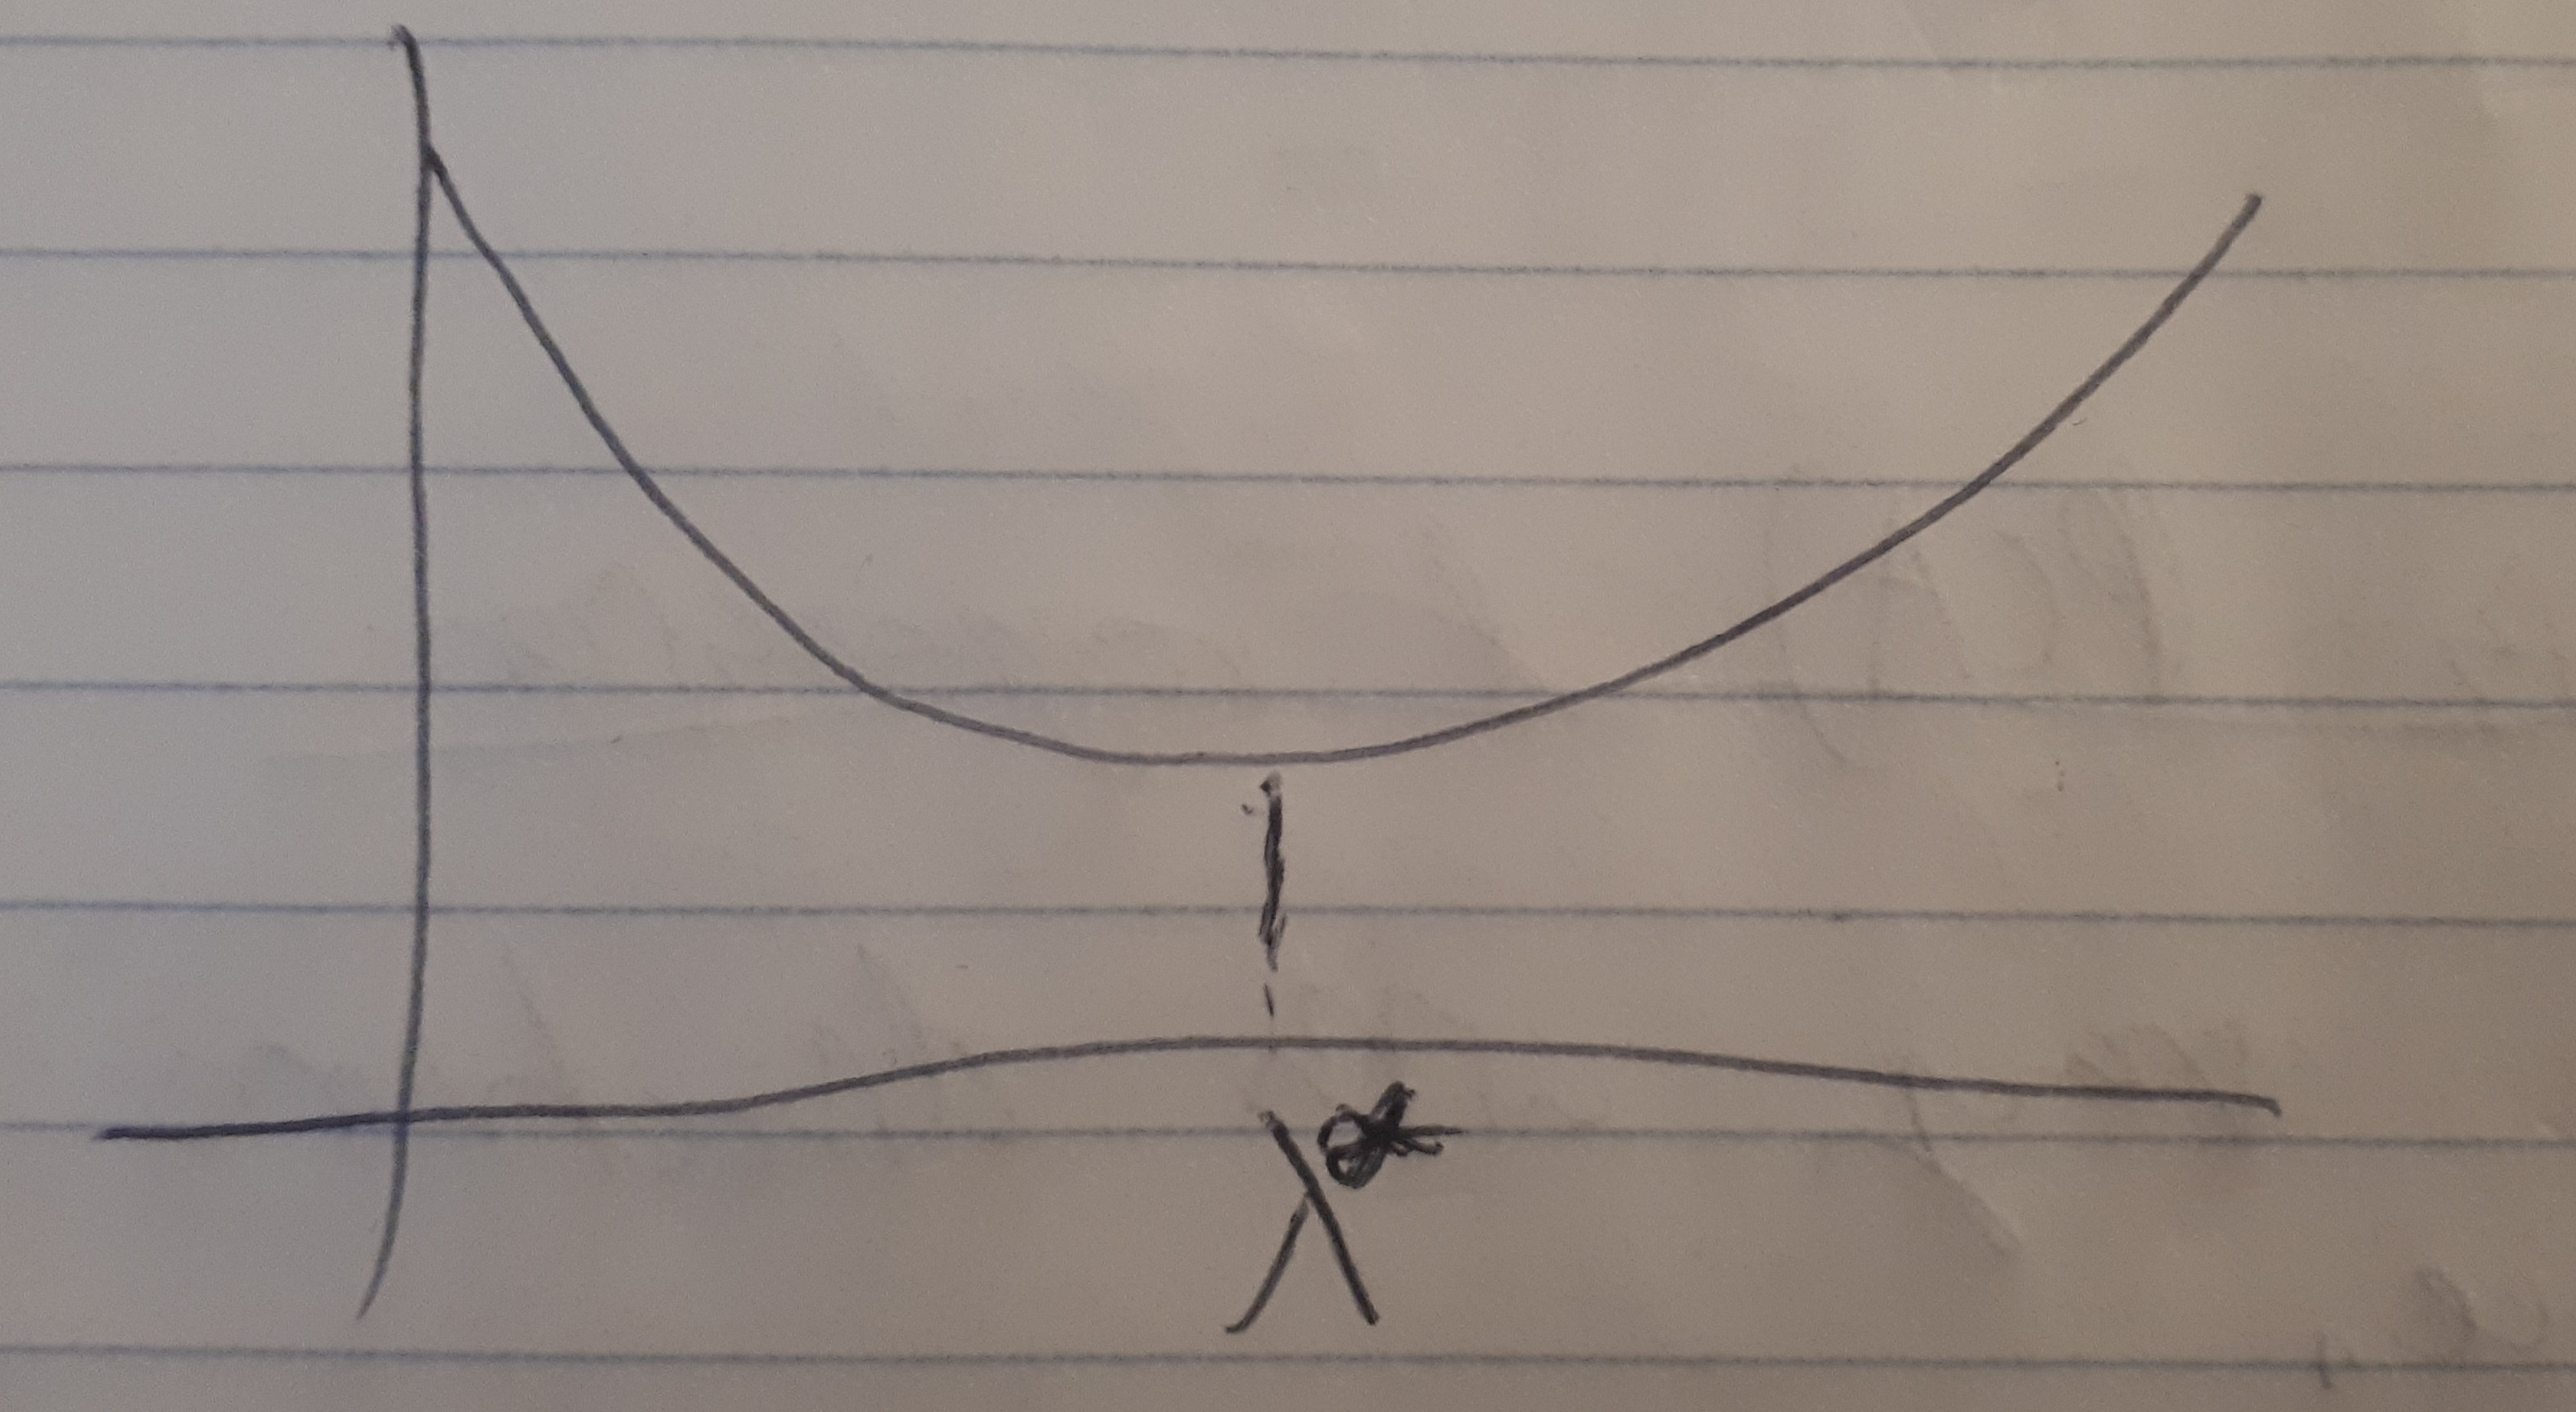
\includegraphics[width = \textwidth/2]{11_04_P02.jpg}
\end{center}
A natural question is can we find $\la^*$? The number $\la^*$ is the value of $\la$ with the smallest risk. We know that 
\[\E[RSS_\la] = nR_{in}(\wh{\beta}_\la) +n\sigma^2 -2\sigma^2 \tr(H_\la). \]
Thus if we can estimate $\sigma^2$ with $\wh{\sigma}^2$, then we can choose $\la$ to minimize
\[\E[RSS_\la] + 2\wh{\sigma}^2 \tr(H_\la).\]
On the homework we will look at different estimators of $\wh{\sigma}^2$.

\subsection{Regularization path}
We often want to compute $\wh{\beta}_\la$ for all $\la \ge 0$. This gives us a path of solutions parametrized by $\la$ which is called a \emph{regularization path}. This can be done very efficiently if we have the SVD of $X$. Suppose $X=U\Gamma V^T$, then
\begin{align*}
    \wh{\beta}_\la &= (X^TX+\la I)^{-1} X^T y \\
    &= V\left(\Gamma^2 +\la I\right)^{-1}\Gamma U^T y\\
    &=\sum_{i=1}^d v_j \frac{\gamma_j}{\gamma_j^2+\la}u_j^T y.
\end{align*}
If we store $\wt{y} = U^Ty$, then we can compute
\[\wh{\beta}_\la = V\diag\left(\frac{\gamma_j}{\gamma_j+\la}\right)\wt{y}, \]
which can be done in $O(d^2)$ time.
\section{Principal component analysis (PCA) and regression}
Idea: Often $y$ should vary with directions in $x$ that have high variance. This is the idea of \emph{principal component analysis (PCA)}: find directions in $X$-space that vary the most (equivalently find direction in $X$-space that most accurately reconstruct our data $\{x_i\}$ ). For example if our data looks like the below picture, we wish to find the blue line.

\begin{center}
    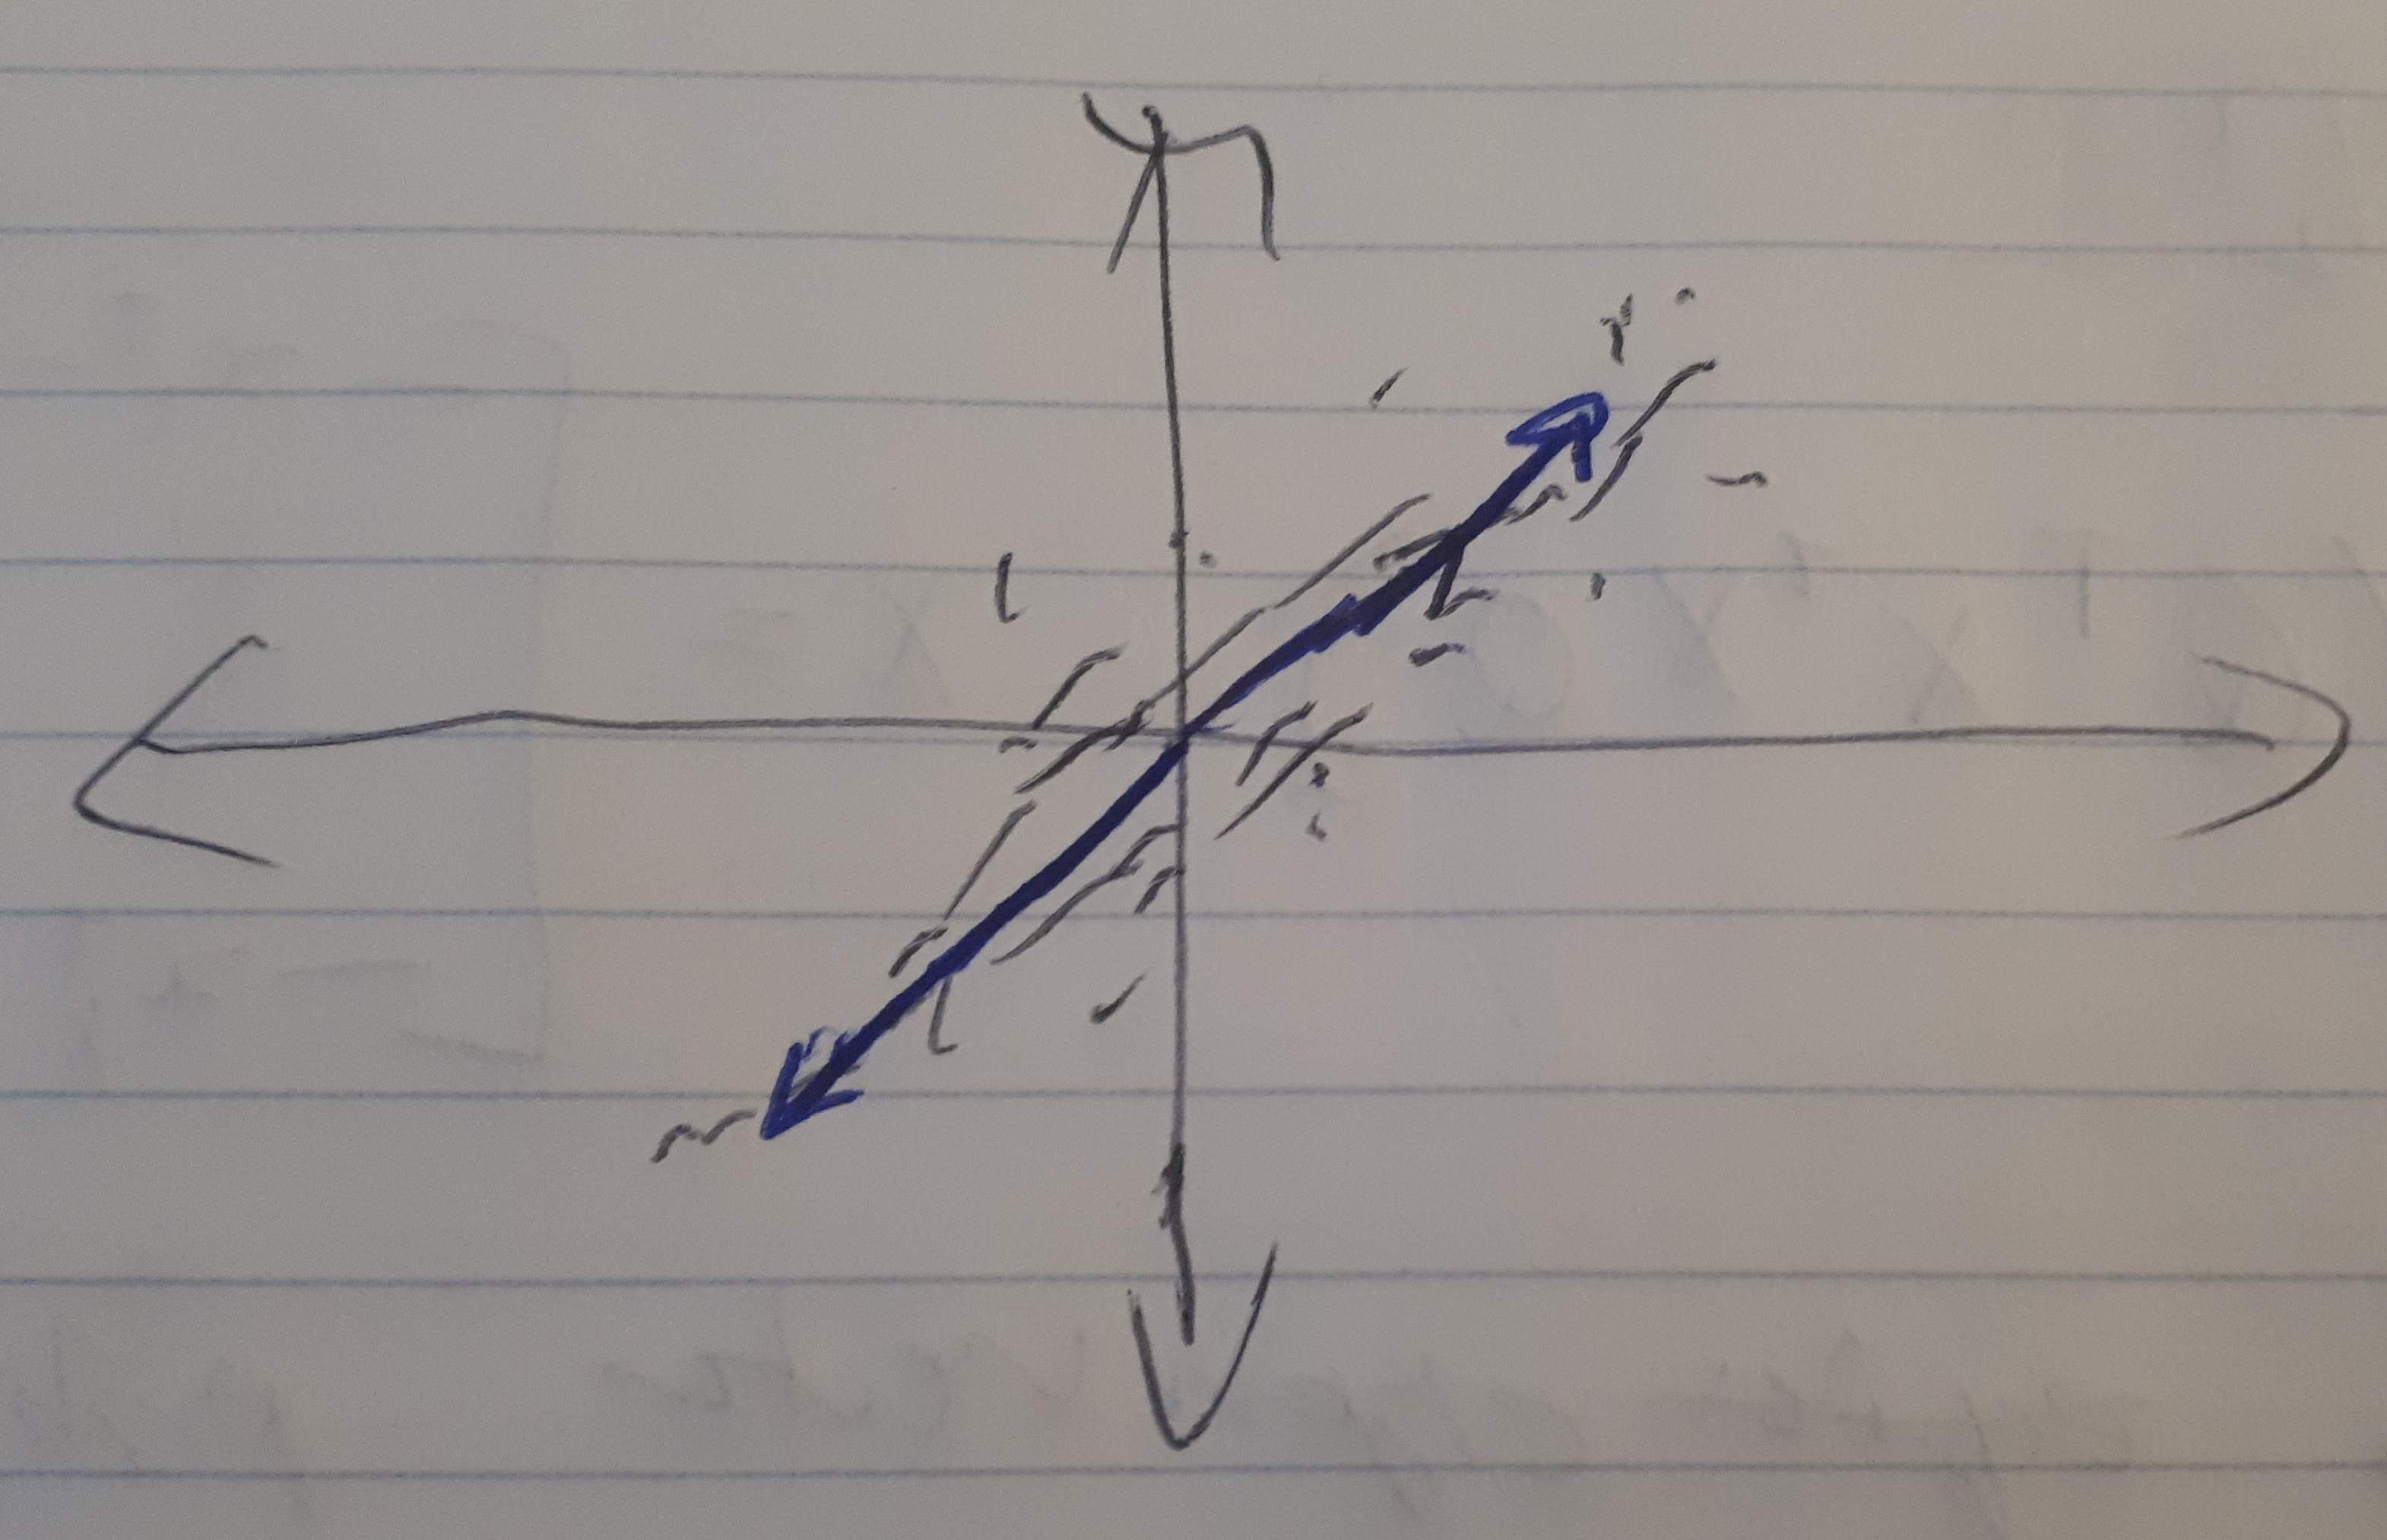
\includegraphics[width = \textwidth/2]{11_04_P03.jpg}
\end{center}

Suppose we have a subspace $\Ss = \spn\{q_1,\ldots, q_k\}$ where $q_i \in \R^d$ are orthonormal, that is
\[q_i^Tq_j = \begin{cases}
    1 & \text{if } i = j,\\
    0 & \text{if } i \neq j.
\end{cases} \]
Then the projection onto $\Ss$ is $\Pi_\Ss = QQ^T$ where $Q = [q_1,\ldots,q_k] \in \R^{d \times k}$. Then for all $x \in \R^d$,
\begin{align*}
    \text{dist}^2(x,\Ss) &= \norm{x-\Pi_\Ss x}_2^2\\
    &= \norm{(I-QQ^T)x}_2^2\\
    &=\norm{x}_2^2-\norm{Q^Tx}_2^2.
\end{align*}
This gives us a procedure for PCA. We wish to find a $k$-dimensional subspace which is closest to all our data $x_1,\ldots, x_n$. Thus we wish to solve
\begin{align*}
    \min_{Q^TQ = I_k} \sum_{i=1}^n \text{dist}^2(x_i, \spn(Q)) &=\min_{Q^TQ=I_k}\sum_{i=1}^n \norm{(I-QQ^T)x_i}_2^2\\
    &=\min_{Q^TQ=I_k}\sum_{i=1}^n \norm{x}-\norm{Q^Tx_i}_2^2\\
    &=\max_{Q^TQ = I_k}\sum_{i=1}^n \norm{Q^T x_i}_2^2 \\
    &= \max_{Q^TQ=I_k} \tr(Q^TX^TXQ),
\end{align*}
where 
\[X = \begin{bmatrix}
    x_1^T\\\vdots \\ x_n^T 
\end{bmatrix} \in \R^{n \times d}.\]
\begin{remark}
    This is an eigenvalue/eigenvector problem. If $X = U\Gamma V^T$, then our problem becomes 
    \[\max_{Q^TQ = I_k} \tr(Q^TV\Gamma^2 V^T Q). \]
    Our idea: put all ``juice'' for the first $k$ directions in $V$ into $Q$ since 
    \[\Gamma^2 = \diag(\gamma_1^2,\ldots, \gamma_d^2), \]
    where $\gamma_1 \ge \ldots \ge \gamma_d$. So $Q=[v_1,\ldots, v_k]$. For reference this concept is called:
    \begin{itemize}
        \item Variational characterization of eigenvectors.
        \item Rayleigh-Ritz eigenvector characterization.
    \end{itemize}
\end{remark}
\end{document}